% Created 2017-10-24 Tue 18:06
\documentclass[11pt]{article}
\usepackage[latin1]{inputenc}
\usepackage[T1]{fontenc}
\usepackage{fixltx2e}
\usepackage{graphicx}
\usepackage{longtable}
\usepackage{float}
\usepackage{wrapfig}
\usepackage{soul}
\usepackage{textcomp}
\usepackage{marvosym}
\usepackage{wasysym}
\usepackage{latexsym}
\usepackage{amssymb}
\usepackage{hyperref}
\tolerance=1000
\providecommand{\alert}[1]{\textbf{#1}}

\title{Virtual Labs Cluster Automation}
\author{SUNANDAN RAJ PULLAGURA}
\date{\today}
\hypersetup{
  pdfkeywords={},
  pdfsubject={},
  pdfcreator={Emacs Org-mode version 7.9.3f}}

\begin{document}

\maketitle

\setcounter{tocdepth}{3}
\tableofcontents
\vspace*{1cm}
\section{Introduction}
\label{sec-1}

  This document is for automating the Virtual Labs cluster setup using
  ansible( Configuration management tool).
\section{Problem}
\label{sec-2}

  The problem is \href{https://bitbucket.org/vlead/systems-model/src/fd77adcc24ad68ce22194fad2224adb12c5219ab/src/bootstrapping.org?at%3Ddevelop&fileviewer%3Dfile-view-default}{bootstrapping} steps for cluster creation. For
  creating VLEAD cluster( Infrastructure for hosting labs),
  bootstrapping steps takes three to four days for VLEAD Employees( who
  knows about VLEAD cluster) and for others it may take two to three
  weeks.
\section{Objective}
\label{sec-3}

  Automate the boostrapping steps and running \href{https://bitbucket.org/vlead/systems-model/src/fd77adcc24ad?at%3Ddevelop}{systems-model} ansible
  playbooks. So that eliminate more number of days to setup VLEAD
  cluster and install cluster in minimal steps in one day.
\section{Network Diagram}
\label{sec-4}

  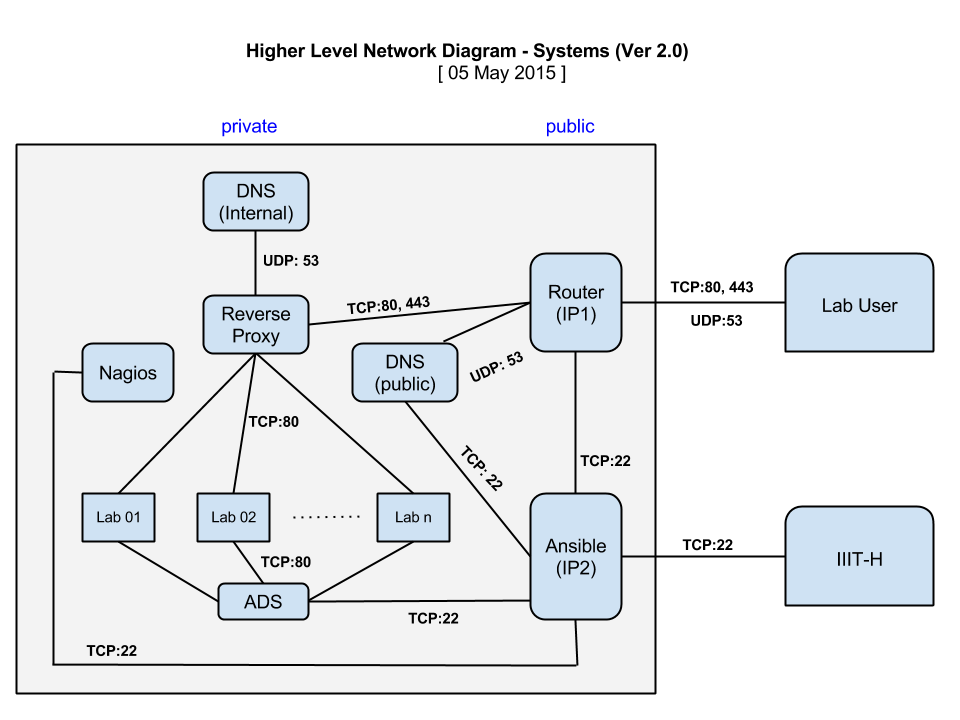
\includegraphics[width=.9\linewidth]{./overall-cluster-network-diagram.png}
\section{Implementation}
\label{sec-5}

\begin{itemize}
\item \href{file://../imp/index.org}{Implementation}
\end{itemize}
\section{Bootstrapping steps}
\label{sec-6}

\begin{itemize}
\item \href{file:///home/sunandan/Desktop/internship/cluster-automation/src/bootstrapping.org}{Bootstrapping steps}
    These steps are needed to setup cluster using ansible scripts
    written in implementation section.
\end{itemize}
\section{Important Repositories}
\label{sec-7}

  The following repositories are used in automation steps which are in github
\begin{itemize}
\item \href{https://github.com/vlead/cluster-automation}{cluster-automation}
\item \href{https://github.com/vlead/cluster-setup-ovpl-centos}{cluster-setup-ovpl-centos}
\item \href{https://bitbucket.org/vlead/systems-model/}{Systems-model}
\end{itemize}
  
\section{Issues and Milestones}
\label{sec-8}

  Links for issues raised during execution and weekly milestones
\begin{itemize}
\item \href{https://github.com/vlead/cluster-automation/issues}{Issues}
\item \href{https://github.com/vlead/cluster-automation/milestones}{Milestones}
\end{itemize}
\section{Branches in cluster-automation repository}
\label{sec-9}

\begin{itemize}
\item Master   - Production repo
\item Develop  - Development repo ( similar to Master)
\item Features - Adding features
\end{itemize}

\end{document}
